\chapter{Methodology}
\section{Time to Digital Converter}

\subsection{specifications}
The main specifications for the TDC are the following:
\begin{itemize}
    \item Clock reference frequency: 100 MHz
    \item Number of bits: 4
    \item Acquisition range: -2$\pi$ to 2$\pi$
\end{itemize}

The TDC implements a 4-bit flash architecture for a time resolution of 625 ps ($\Delta$) in each half of the clock period. The acquisition range is 20 ns, which corresponds to a phase 
range of -2$\pi$ to 2$\pi$ for a clock frequency of 100 MHz.

\subsection{Architecture}
The TDC architecture is based on the design presented in \cite{bib:tdc_flash}. The core of the TDC consist of a voltage-controlled delay line (VCDL), a set of D flip-flops to sample the
state of the VCDL, and a thermometer-to-binary decoder that process the sampled data to produce a workable digital output. This arrangement is used twice, once for the case when the
feedback signal has a lower frequency (or delayed phase) than the reference clock, and the other for the case when the feedback signal has a higher frequency (or advanced phase) than
the reference clock. The two outputs are then combined to produce the final output of the TDC. Such an architecture (Fig. \ref{fig:TDC_conventional_architecture}) would be the 
conventional way to implement a TDC that reads both cases for the phase difference between the reference clock and the feedback signal. 

\begin{figure}[h]
    \centering
    \includegraphics[width=1\textwidth]{figures/TDC_conventional_architecture.png}
    \caption{Conventional TDC architecture}
    \label{fig:TDC_conventional_architecture}
\end{figure}

The architecture of figure \ref{fig:TDC_conventional_architecture} has shortcomings, such as the fact that it does not allow for a phase difference of more than 2$\pi$ between the
reference clock and the feedback signal, meaning that the TDC will not be able to read the phase difference beyond half cycle for each clock period. This is limiting for the PLL, as it
would not be able to correct the phase difference if it exceeds $\pi$ for each case. To overcome this limitation and achieve the desired acquisition range set in the specifications, 
the TDC architecture of figure \ref{fig:TDC_proposed_architecture} is proposed.

\begin{figure}[h]
    \centering
    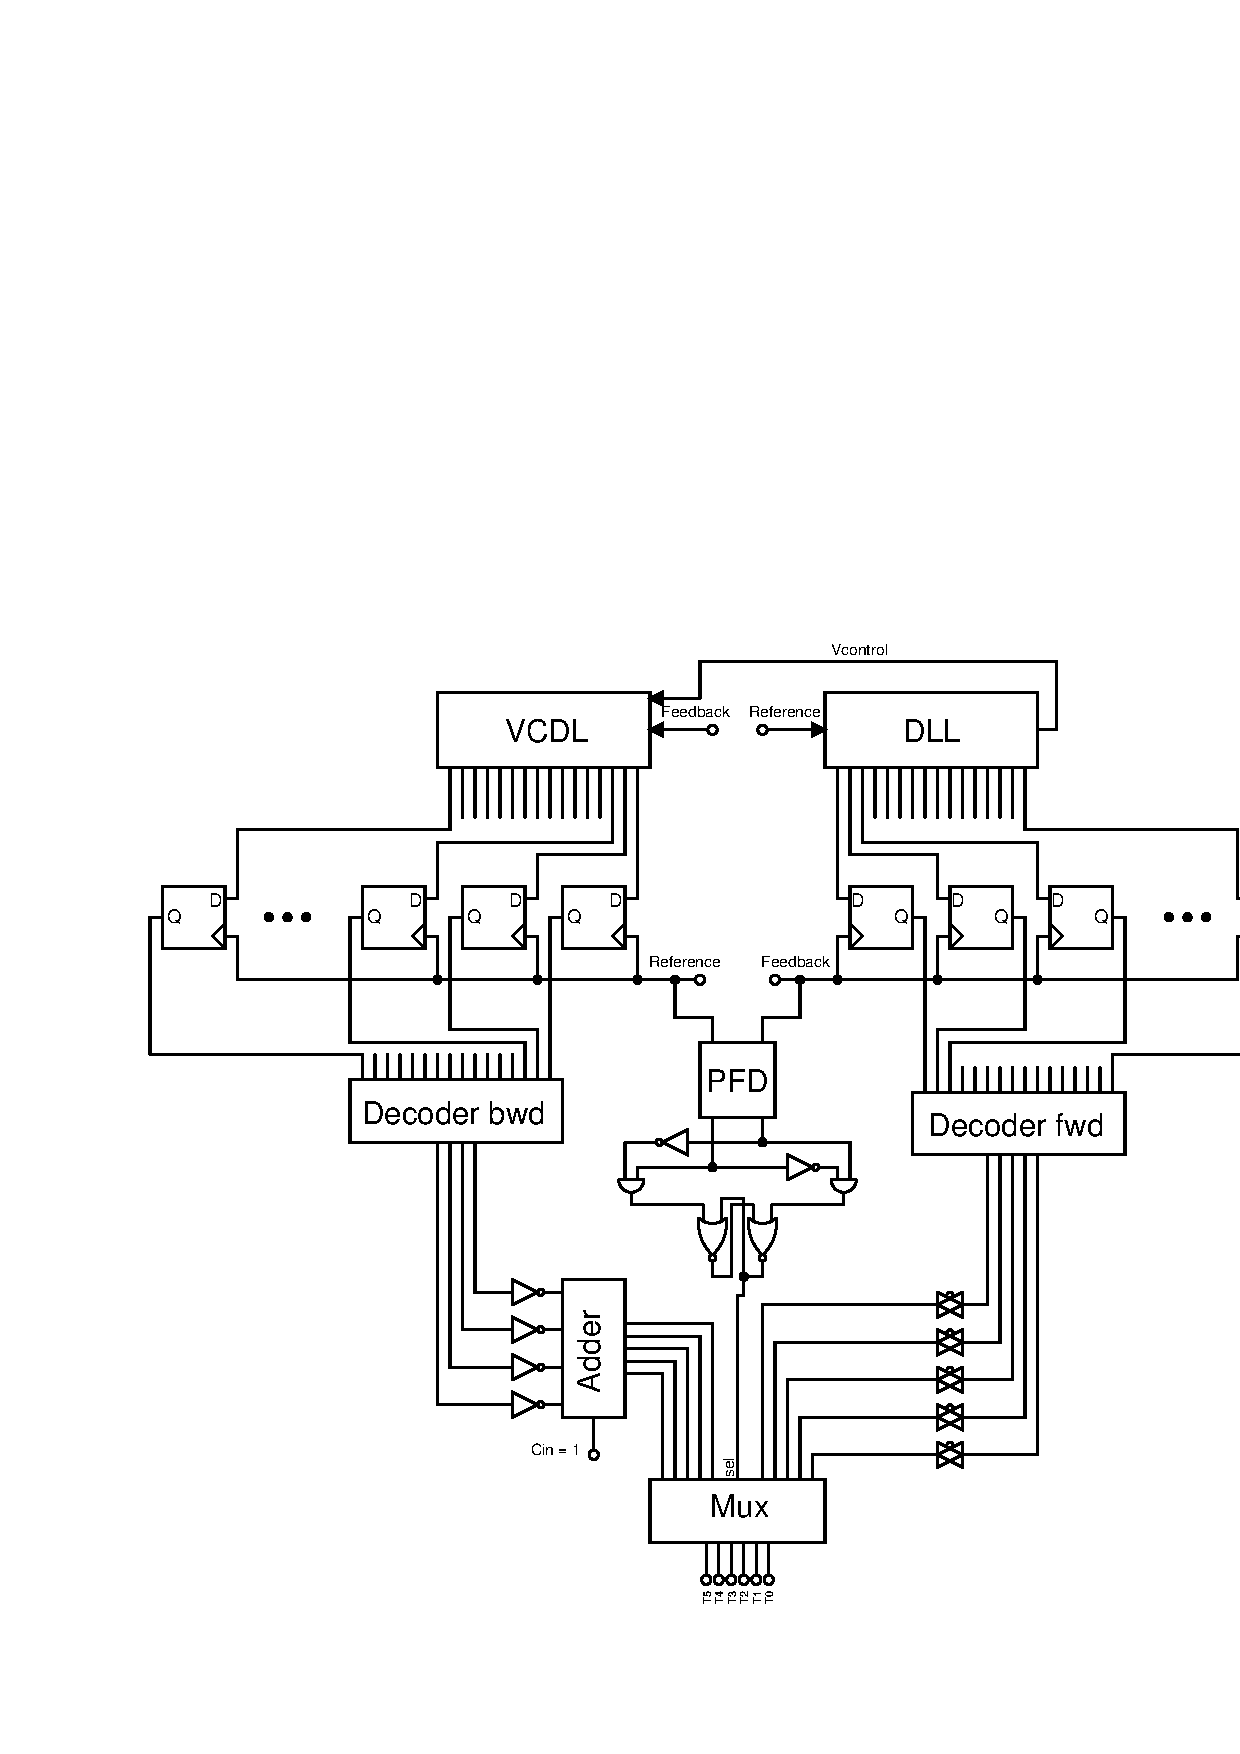
\includegraphics[width=1\textwidth]{figures/TDC_proposed_architecture.png}
    \caption{Proposed TDC architecture}
    \label{fig:TDC_proposed_architecture}
\end{figure}

The main differences between the conventional architecture and the proposed one are that the latter uses a DLL instead of a VCDL to implement the delay line, a slight modification
to the thermometer-to-binary decoder, and a different way to combine the outputs of the two TDCs.

The DLL allows for a more robust and stable delay line as it is less sensitive to PVT variations. This is important for the PLL, as it needs to be able to operate under different
conditions and still be able to correct the phase difference between the reference clock and the feedback signal.

The thermometer-to-binary decoder is modified to allow for the reading of both cases of the phase/frequency difference between the signals. This is the main way that the TDC is able
to read a phase difference of more than 2$\pi$ each cycle and as far as the author is aware, this is the first time that such a modification has been proposed in the literature.

Finally, the outputs of the two TDCs are combined using a multiplexer that selects the output based on the frequency state of the feedback signal. The selector needs to be able to
determine whether the feedback signal is leading or lagging the reference clock, which is done by retrieving the frequency information that was lost because of the decoder modification.


All of this changes done to the conventional TDC architecture will be further explained in the following sections of this chapter, where the design of the TDC will be presented in 
detail.

\subsection{Design}

\section{Digitally controlled oscillator}

\section{Digital loop filter}
